\documentclass{article}

% if you need to pass options to natbib, use, e.g.:
%     \PassOptionsToPackage{numbers, compress}{natbib}
% before loading neurips_2018

% ready for submission
% \usepackage{neurips_2018}

% to compile a preprint version, e.g., for submission to arXiv, add add the
% [preprint] option:
%     \usepackage[preprint]{neurips_2018}

% to compile a camera-ready version, add the [final] option, e.g.:
     \usepackage[final]{nips_2018}

% to avoid loading the natbib package, add option nonatbib:
%     \usepackage[nonatbib]{neurips_2018}

\usepackage[utf8]{inputenc} % allow utf-8 input
\usepackage[T1]{fontenc}    % use 8-bit T1 fonts
\usepackage{hyperref}       % hyperlinks
\usepackage{url}            % simple URL typesetting
\usepackage{booktabs}       % professional-quality tables
\usepackage{amsfonts}       % blackboard math symbols
\usepackage{nicefrac}       % compact symbols for 1/2, etc.
\usepackage{microtype}      % microtypography
\usepackage{graphicx}      % microtypography

\title{Exploring Different Approaches to Improve Binary Classification Performance for Imbalanced Data Set}

% The \author macro works with any number of authors. There are two commands
% used to separate the names and addresses of multiple authors: \And and \AND.
%
% Using \And between authors leaves it to LaTeX to determine where to break the
% lines. Using \AND forces a line break at that point. So, if LaTeX puts 3 of 4
% authors names on the first line, and the last on the second line, try using
% \AND instead of \And before the third author name.

\author{%
  Yuan Sun\\
  Department of Computer Engineering\\
  University of British Columbia\\
  Vancouver, BC\\
  \texttt{round.sun@alumni.ubc.ca}\\
  \And
  Yixuan Ji\\
  Department of Computer Engineering\\
  University of British Columbia\\
  Vancouver, BC\\
  \texttt{jiyixuan@ece.ubc.ca}\\
  \AND
  Jay Fu\\
  Department of Computer Engineering\\
  University of British Columbia\\
  Vancouver, BC\\
  \texttt{jay.fu@alumni.ubc.ca}\\
}

\begin{document}
% \nipsfinalcopy is no longer used

\maketitle

\begin{abstract}
It is common to find imbalanced datasets in a wide range of applications in human society. With the development of modern machine learning and data science, the imbalanced feature of datasets is becoming more and more significant and meaningful in terms of binary classification. Therefore, exploring various approaches with higher accuracy for manipulating imbalanced datasets is a critical topic which should be focused on. In this work, we use multiple novel approaches in sampling\&modeling and compare the performance of handling imbalanced datasets with existing method for binary classification. In addition, we discuss relevant studies in this field in detail and compare our results with theirs, which would indicate a potential direction in the future.
\end{abstract}

\section{Introduction}
which could often bring a convenient way of handling similar things efficiently in the future. Binary classification a typical and commonly used classification method. The performance of binary classification could have a profound influence for people’s daily life, such as credit risk assessment, medical diagnosis for patients [2], food quality evaluation, etc. However, the existing method of fitting imbalanced dataset for binary classification model would always have drawbacks. Because they barely combine the various ensemble methods and multiple sampling techniques together, although there are some works applying specific ensemble method into over/under sampling [3]. Therefore, there are some blank spaces in this field we can explore and compare to find an optimum approach for binary classification.
\\\\It is self-evident that significance of binary classification is growing day by day in multiple areas of study. Mapping distribution, disturbance, wildlife habit, fire risk and climate change [4] are all relying on binary classification. What’s more, multiple classification problems could also be deduced as binary classification problems, such as one versus all classification which is as accurate as any other approach [5]. Nevertheless, the imbalanced data set would often result in a relative less accurate model. This concern is essential in real world applications as well, such as information retrieval, text categorization and filtering tasks [6].
\\\\Through empirical analysis, we know that fitting the imbalanced dataset into machine learning(ML) models would always give various limitations and constraints. For the imbalanced datasets, how could people know the variations among those different techniques or ensemble model in terms of binary classification? Will the performance be improved if the best-performed sampling technique are utilized together to ensemble method? There are obviously some improvements and quantized comparisons can be presented to help people to select appropriate techniques and ensemble models.
\\\\In this work, we firstly apply three techniques which are oversampling, undersampling and class weighting into our original dataset and derive three modified datasets. Based on these modified datasets, we respectively explore the performance of models with those three datasets and compare the results with existing work. Secondly, we use different ensemble methods with datasets and try to find the most suitable one. Finally, we combine the well-performed techniques and ensemble methods together to explore the framework with the best performance.


\section{Related Work}
\label{gen_inst}
\subsection{Benchmarking binary classification models with different degrees of imbalanace}

This paper mainly focus on handling the variation among a wide range of models and compare the accuracy (test error) between those models in terms of the degree of imbalance. We use the notation $x = (x_1, x_2,...,x_m)^T$ to represent the a set of $m$ variables that describe an instance. Each variable for a particular instance $k$ can be denoted by $x_k = (x_k1, x_k2,...,x_km)^T$ [2]. And the output $y_k \in \{-1, +1\}$. The degrees of imbalance determines how biased the dataset set could be for a binary classification. Based on the previous work of imbalanced dataset[7], this paper investigate the influence of degrees of imbalance for lots of models. However, this paper only simply use models to evaluate accuracy for imbalanced datasets. Besides ensemble models, our work includes more techniques such as oversampling, undersampling and class weighting.

\subsection{Imbalanced datasets with SVM Ensembles}
SVMs have gained remarkable success in a wide range of applications, in the imbalanced data context. This study proposed to combine integrated sampling techniques with an ensemble of SVMs[8]. The effects of class imbalance on SVMs have been conducted on this paper.
\begin{figure}
  \centering
  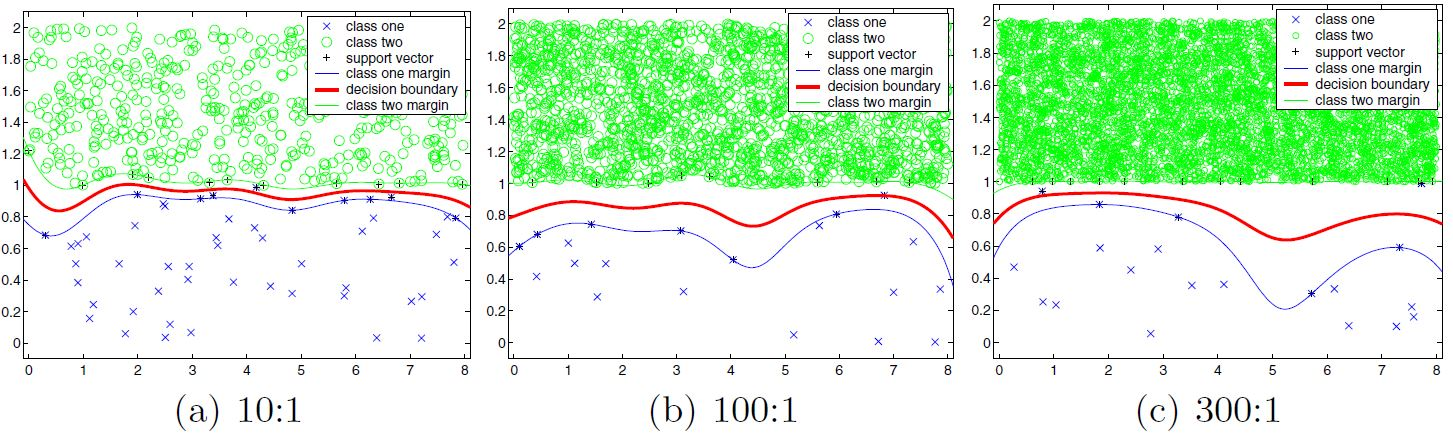
\includegraphics[width=\linewidth]{../fig/imbalanced_data.JPG}
  \caption{Boundary changes wiht different imbalance ratios[8]}
  \label{Boundary}
\end{figure}
\\\\From the Figure ~\ref{Boundary}, we can clearly see that the difference between ideal boundary and real boundary is moderate when the imbalanced ratio is relatively small [8]. Nevertheless, the boundaries move towards the minority class when the ratio is getting higher and higher. Given this phenomenon, the paper tries to solve this problem by using sampling techniques to balance the data.
There are still some more spaces left for us to explore, although sampling techniques are used for this framework. Besides for sampling techniques, we still add class weighting method into our framework with different ensemble approaches. In this case, we make more comparisons and explorations under multiple conditions.

\subsection{Using an ensemble method for imbalanced medical data classification}
In this study, it mainly presents its solution for KDD Cup 2008 competition which aims at optimizing the detection for breast cancer [9]. Class-Balanced SVM is the main tool used in this study. Besides, this study exploited weighted-based classification method specifically for medical imbalanced dataset. This typical feature of medical dataset is that the number of samples is normally small and the dimensionality is high [10]. Therefore, this study tries to integrate SVM, AdaBoost and GA to solve imbalanced medical data problem. The ensemble method used in this paper [9] is adequate enough, whereas it doesn’t apply targeted pre-processing of data into framework. In our work, we pre-process that original dataset and apply multiple approaches to the model, such as undersampling, oversampling and class weighting.

\section{Descriptions and Justifications}
\label{headings}

To boost up the accuracy of a model and minimize the effect of imbalanced data on the performance, there are several possible solutions, including undersampling, oversampling and class weighting. However, seldom have studied the difference in these approaches. The motivation of this experiment is to study how different machine learning techniques could have impact on the performance of models trained on imbalanced data set. The following sections discuss in detail the settings of the experiment and some of the approaches to tackle imbalanced problems.

\subsection{Data Set Settings}
The data set is drawn from the UCI Machine Learning Repository and is publicly known as the $Adult$ data set [1]. It contains general information of 48843 individuals and whether or not they make more than 50K every year. The goal is to build a model that can accurately predict the annual income ($>50K$ or $<=50K$) of a given person based on this data set. As shown in Table~\ref{attributes}, the data set contains a mixture of categorical and numerical features for each entry. Therefore, data pre-processing techniques should be applied to enable further study on the data. Specifically, feature selecion algorithms could help decide which features are relevant to the prediction. In addition, the label $salary$ is a binary attribute of the individual's income being either $>50K$ or $<=50K$, which makes it an ideal binary classification problems.\\\\
The major challenge for this data set is the imbalance of its binary label. There are only 11687 positive ($>50K$) labels out of 48843 entries in total, which makes up $23.9\%$ of the whole data set. Models trained on imbalanced data set tend to make prediction of the majority class. For example, consider a data set consisting $10000$ entries of class $A$ and $100$ entries of class $B$. The model could get 90\% of training accuracy by simply predicting everything as class $A$. The following sections discuss several methods to handle imbalanced data set, including previous efforts that has been made to study this data set, as well as other machine learning techniques that could also be applied.

\begin{table}
  \caption{$Adult$ Data Set Attributes [1]}
  \label{attributes}
  \centering
  \begin{tabular}{ll}
    \toprule
    Name     & Description\\
    \midrule
    Age & Continuous\\
    Workclass & Private, Self-emp-not-inc, Self-emp-inc, Federal-gov, Local-gov,\\ &State-gov, Without-pay, Never-worked\\
    Final Weight & The number of people the census believes the entry represents; Continuous\\
    Education & Bachelors, Some-college, 11th, HS-grad, Prof-school, Assoc-acdm, \\&Assoc-voc, 9th, 7th-8th, 12th, Masters, 1st-4th, 10th, Doctorate, 5th-6th, \\&Preschool\\
    Education-Num & Continuous\\
    Marital-Status & Married-civ-spouse, Divorced, Never-married, Separated, Widowed, \\&Married-spouse-absent, Married-AF-spouse\\
    Occupation & Tech-support, Craft-repair, Other-service, Sales, Exec-managerial, \\&Prof-specialty, Handlers-cleaners, Machine-op-inspct, Adm-clerical, \\&Farming-fishing, Transport-moving, Priv-house-serv, Protective-serv, \\&Armed-Forces\\
    Relationship & Wife, Own-child, Husband, Not-in-family, Other-relative, Unmarried\\
    Race & White, Asian-Pac-Islander, Amer-Indian-Eskimo, Other, Black\\
    Sex & Female, Male\\
    Capital-Gain & Continuous\\
    Capital-Loss & Continuous\\
    Hours-per-Week & Continuous\\
    Native-Country & United-States, Cambodia, England, Puerto-Rico, Canada, Germany, \\&Outlying-US(Guam-USVI-etc), India, Japan, Greece, South, China, Cuba, \\&Iran, Honduras, Philippines, Italy, Poland, Jamaica, Vietnam, Mexico, \\&Portugal, Ireland, France, Dominican-Republic, Laos, Ecuador, Taiwan, \\&Haiti, Columbia, Hungary, Guatemala, Nicaragua, Scotland, Thailand, \\&Yugoslavia, El-Salvador, Trinadad\& Tobago, Peru, Hong, \\&Holand-Netherlands\\
    Salary & >50K, <=50K\\
    \bottomrule
  \end{tabular}
\end{table}

\subsection{Mearsure of Performance}
\label{measure_of_performance}

In order to compare different algorithms, let us first define the measure of performance. In the sense of binary classification, predictions can be categorized into four different types: true positive (TP), false positive (FP), true negative (TN) and false negative (FP). In different applictions, performance can be measured using different formulae. The following three are the most used formulae [4] in binary classification:\\
\begin{center}
\hfill$Sensitivity (SEN)=\frac{TP}{TP+FP}$\hfill (1)\\\hfill\\
\hfill$Specificity (SPE)=\frac{TN}{TN+FN}$\hfill (2)\\\hfill\\
\hfill$Predictive Accuracy (PA)=\frac{TP+TN}{TP+FP+TN+FN}$\hfill (3)\\
\end{center}
$Sensitivity$ focuses on the model's accuracy on its positive predictions whereas $specificity$ focuses on negative predictions. $Predictive accuracy$ on the other hand, is used to measure the general accuracy of the model over both positive and negative predictions. In this experiments, we compare the performance of different algoritms using all three of the measures.

\subsection{Undersampling}
\label{undersampling}

One of the most popular methods in handling imbalanced data sets is data undersampling, in which entries are randomly sampled from the majority class. Only a portion of the majority class are collected such that the size of the sampled majority class is the same as the minority class. Inouye (2018) has implemented such sampling method to the $Adult$ data set [5]. He randomly generated a subset of sample with income $<=50K$ and simply discarded the rest. This approach usually works relatively well, however, massive amount of data is discarded and the resulted model would not be able to reflect the comlete data set. Next section introduces an alternative method that could potentially utilize every entry of the data set to build the model.

\subsection{Oversampling}
\label{oversampling}

As an alternative to the undersampling method, oversampling "creates" new entries of the minority class to match the size of majority class. The simplest way to oversample is to duplicate the minority class multiple times. However, there are more sophisticated oversampling algorithms, such as SMOTE and ADASYN, that can create synthetic data points as oppose to duplicating original entries. The particular algorithm used in this experiment is ADASYN, which randomly generates a data point based on $k$ nearest neighbors. In addition, ADASYN attributes more weights to data points that are harder to learn [3]. Both undersampling and oversampling are types of data pre-processing methods to solve imbalance problems. Next section introduces another technique that could be applied in the training phase of model fitting.

\subsection{Class Weighting}
\label{class_weighting}

Class weighting is a method that assigns more weights on important classes so that the model focuses more on one class than the other during training. This method can also be applied to imbalanced data set so the model would focus more on the minority class. Lo, et al. (2008) applied class-balanced support vector machine (CB-SVM) to solve imbalanced problems [2]. They assigned different weights to each class to prevent the model from favoring majority class. Similarly, class weighting is also conducted in this experiment using the $svm$ module in $scikit-learn$ package. The specific function used, $SVC$, allows users to specify weights for each class through the parameter $class\_weight$.

\subsection{Ensemble}
\label{ensemble}

Another approach that could potentially enhance the performance is model ensembling. In general it could help reduce the training error and/or approximation error of a variety of problems. However, seldom have applied ensemble method to the $adult$ data set. In this experiment, we apply ensemble method to reduce false predictions of the model. Specifically, we gather the outputs of a serie of heterogeneous machine learning models and train another logistic regression model based on these outputs. This is known as the stacking ensemble method. Section~\ref{experiments} discusses in detail how different techniques, including ensemble methods, would impact on the performance.

\section{Experiments}
\label{experiments}

We have done two experiments to study the effects of data balancing techniques and ensemble methods on performance. All hyper-parameters used in this section are determined using 10-fold cross validation. After shuffling the raw data set, we devide it into training set and testing set by a ratio of $7:3$. All algorithms use the same training set and test set for comparison purposes. In addition, we perform one-hot encoding to all categorical features. In particular, for the missing categorical data, one-hot representation would simply be all zeros. And missing numerical data is filled with average of the corresponding feature column.

\subsection{Data Balancing Techniques}
\label{balancing_experiment}

The first experiment is to compare the performance of models after applying three different data balancing techniques as previously introduced: undersampling, oversampling and class weighting. In order to study only the effects of these techniques, we have controlled as many variables as possible. All three techniques use the same $adult$ data set and same machine learning algorithms with the same hyper-parameters. In order to better observe how each technique influence the result, we conduct another control group in which no data balancing techniques are used. See Table~\ref{balancing} for the performance of each algorithms using different balancing techniques. As introduced in Section~\ref{measure_of_performance}, binary classification models can be measured using SEN, SPE and PA. The corresponding scores are presented in the table.\\

As shown,

\begin{table}
  \caption{Data Balancing Techniques}
  \label{balancing}
  \centering
  \begin{tabular}{ll}
    \toprule
    Algorithm & 
    	\begin{tabular}{llll}
    		\hfil Undersampling&\hfil Oversampling&\hfil Class Weighting&\hfil None\\
    		\midrule
    		\begin{tabular}{lll} SEN&SPE&PA \end{tabular}&
    		\begin{tabular}{lll} SEN&SPE&PA \end{tabular}&
    		\begin{tabular}{lll} SEN&SPE&PA \end{tabular}&
    		\begin{tabular}{lll} SEN&SPE&PA \end{tabular}
    	\end{tabular}\\
    \midrule
    Age &\begin{tabular}{llll}
    	\begin{tabular}{lll} 999&988&100 \end{tabular}&
    	\begin{tabular}{lll} 999&988888&100 \end{tabular}&
    	\begin{tabular}{lll} 999&988&100 \end{tabular}&
    	\begin{tabular}{lll} 999&988&100 \end{tabular}
    \end{tabular}\\
    
    Age &\begin{tabular}{llll}
    	\begin{tabular}{lll} 999&988&100 \end{tabular}&
    	\begin{tabular}{lll} 999&988888&100 \end{tabular}&
    	\begin{tabular}{lll} 999&988&100 \end{tabular}&
    	\begin{tabular}{lll} 999&988&100 \end{tabular}
    \end{tabular}\\
    
    Age &\begin{tabular}{llll}
    	\begin{tabular}{lll} 999&988&100 \end{tabular}&
    	\begin{tabular}{lll} 999&988888&100 \end{tabular}&
    	\begin{tabular}{lll} 999&988&100 \end{tabular}&
    	\begin{tabular}{lll} 999&988&100 \end{tabular}
    \end{tabular}\\
    
    Age &\begin{tabular}{llll}
    	\begin{tabular}{lll} 999&988&100 \end{tabular}&
    	\begin{tabular}{lll} 999&988888&100 \end{tabular}&
    	\begin{tabular}{lll} 999&988&100 \end{tabular}&
    	\begin{tabular}{lll} 999&988&100 \end{tabular}
    \end{tabular}\\
    
    Age &\begin{tabular}{llll}
    	\begin{tabular}{lll} 999&988&100 \end{tabular}&
    	\begin{tabular}{lll} 999&988888&100 \end{tabular}&
    	\begin{tabular}{lll} 999&988&100 \end{tabular}&
    	\begin{tabular}{lll} 999&988&100 \end{tabular}
    \end{tabular}\\
    
    \bottomrule
  \end{tabular}
\end{table}

\subsection{Ensemble Method}

The second experiment explores how ensemble method can affect the model performance. From the result of Section~\ref{balancing_experiment}, we determine that ??? performs the best in this binary data set. Therefore ??? is used in both groups of this experiment in order to control experimental factors. Similar to the previous part, models are compared in three different matrices SEN, SPE and PA.

\begin{table}
  \caption{Ensemble vs. Single Models}
  \label{ensemble_table}
  \centering
  \begin{tabular}{ll}
    \toprule
    Model     & \begin{tabular}{lll} SEN&SPE&PA \end{tabular} \\
    \midrule
    Stacking Ensemble& \begin{tabular}{lll} 9999&9999&8888 \end{tabular} \\
    Model     & \begin{tabular}{lll} SEN&SPE&PA \end{tabular} \\
    Model     & \begin{tabular}{lll} SEN&SPE&PA \end{tabular} \\
    Model     & \begin{tabular}{lll} SEN&SPE&PA \end{tabular} \\
    Model     & \begin{tabular}{lll} SEN&SPE&PA \end{tabular} \\
    Model     & \begin{tabular}{lll} SEN&SPE&PA \end{tabular} \\
    Model     & \begin{tabular}{lll} SEN&SPE&PA \end{tabular} \\
    Model     & \begin{tabular}{lll} SEN&SPE&PA \end{tabular} \\
    \bottomrule
  \end{tabular}
\end{table}

\section{Discussion}

This is the conclusion.\\

One of the major contribution of this experiment is that our work has provided some insights to the performance of different balancing techniques.

In the ensemble experiment, we only used ??? in both groups to control experimental factors. However this might neglect the possibility that a diiferent balancing technique might make a difference in the ensemble results. If time permits, one possible improvement is to conduct ensembling to all balancing techniques and study their difference.

Another potential future improvement is to expand the experiment to more data sets that have different imbalance ratio. This could help explore how balancing techniques and ensemble methods would perform differently with different imbalance ratio.

\section*{References}

\medskip

\small

[1] Kohavi, R.\ \& Becker, B.\ (1996) Adult Data Set.\ {\it UC Irvine Machine Learning Repository},
pp.\ University of California.

[2] Lo, H.Y.\ et al.\ (2008) Learning to Improve Area-Under-FROC for Imbalanced Medical Data Classification Using an Ensemble Method.\ {\it SIGKDD Explorations},
10(2)\ 43--46.

[3] He, H.\ et al.\ (2008) ADASYN: Adaptive Synthetic Sampling Approach for Imbalanced
Learning.\ {\it 2008 International Joint Conference on Neural Networks}, 978-1-4244-1821-3/08. Universidad de Granada.

[4] Zhou, L.\ \& Lai, K.K.\ (2009) Benchmarking binary classification models on data sets with different degrees of imbalance.\ {\it Front. Comput. Sci. China 2009},
3(2)\ 205--216.

[5] Inouye, S.\ (2018) Census Income Classification in R.\ {\it Inertia7}.

\end{document}
